%%% Lecture 1

\renewcommand{\thechapter}{\Roman{chapter}}

\chapter{Hurewicz Theorem}

\section{Introduction}

\lecture[Introduction and first encounter with Hurewicz theorem.]{2021-10-11}

In the Topology I class given by Prof. Schwede last year, two important homotopy invariant functors were defined:

\begin{itemize}
    \item The singular homology groups $H_n(X;\Z)$. The definition of these groups is quite involved, but they are relatively easy to compute (e.g. by cellular homology). In the case of the spheres we have:
    \[\til{H}_n(S^k;\Z)=\begin{cases*}\Z & if $n=k$ \\ 0 & otherwise\end{cases*}\]
    
    \item The homotopy groups $\pi_n(S^k,*)$. These groups are instead easy to define, but really difficult to compute. In the case of the spheres their calculation becomes complicated already for $n>k$:
    \[\pi_n(S^k)=\begin{cases*}0 & if $n<k$ \\ \Z & if $n=k$ \\ ??? & if $n>k$\end{cases*}\]
    
    As of today (and most likely as of tomorrow too) still a lot is unknown about the higher homotopy groups of the spheres, and those we do know display an apparently erratic behaviour.
\end{itemize}

Homotopy groups are so hard to compute in general that, as a matter of fact, \emph{there is no non-contractible, simply connected finite CW-complex for which all homotopy groups are known.}

\section{A First Look to Hurewicz Theorem}

An important result about homotopy groups is a theorem due to Hurewicz relating the first non-trivial homotopy and homology groups under certain hypotheses:

\begin{theorem}[Hurewicz]\label{theorem:absolute-hurewicz}
Let $n\geq2$ and let $X$ be an $(n-1)$-connected based space. Then $H_i(X;A)=0$ for all $0<i<n$ and any abelian group $A$ and the Hurewicz map
\[h:\pi_n(X,x_0)\to H_n(X;\Z)\]
is an isomorphism.
\end{theorem}

Where the \textbf{Hurewicz map} is defined in the following way. Let $n\geq1$ and let $c\in H_n(S^n;\Z)$ be a generator. For a based space $(X,x_0)$ define
\[h:\pi_n(X,x_0)\to H_n(X;\Z),\ [f:S^n\to X]\mapsto f_*(c)\]
where $f_*:H_n(S^n;\Z)\to H_n(X,\Z)$ is the map induced by $f$ on homology groups. I.e. the Hurewicz map $h$ is the evaluation at the fundamental class of $S^n$.

Proving this theorem will keep us busy for the next few lectures.

\begin{remark}
Choosing the other generator of $H^n(S^n;\Z)$, the Hurewicz map changes into its negative which is still an isomorphism, i.e. the map itself slightly depends on the choice of the generator, but the fact that it is an isomorphism does not.
\end{remark}

\begin{remark}
Recall: for path connected $X$, $h:\pi_1(X,x_0)\to H_1(X,\Z)$ is surjective with kernel the commutator subgroup, so it factors to an isomorphism $\pi_1(X,x_0)^{\text{ab}}\to H_1(X;\Z)$. The Hurewicz theorem is a generalization of this fact, whose first proof is due to Poincaré.
\end{remark}

We know prove two properties of the Hurewicz map, namely its naturality and the fact that it is actually a group homomorphism.

\unnumpar{Naturality of the Hurewicz map} Let $f:X\to Y$ be a based map between based spaces. Then the following square commutes
\begin{center}
    \begin{tikzcd}
        \pi_n(X,x_0) \arrow[r, "h^X"] \arrow[d, "f_*"] & H_n(X;\Z) \arrow[d, "f_*"] \\
        \pi_n(Y,f(x_0)) \arrow[r, "h^Y"] & \pi_n(Y;\Z)
    \end{tikzcd}
\end{center}

\begin{proof}
Let $\alpha:S^n\to X$ represent a class in $\pi_n(X,x_0)$. Then
\[f_*(h^X[\alpha])=f_*(\alpha_*(c))=(f\alpha)_*(c)=h^Y[f\circ\alpha]=h^Y(f_*[\alpha])\]
\end{proof}

\unnumpar{The Hurewicz map is a group homomorphism} Let $p:S^n\to S^n\vee S^n$ be a pinch map\marginnote{\footnotesize The pinch map is the subject of one of the exercises in the first exercise sheet ("The" pinch map, because as we will see it is unique up to homotopy).}, i.e. a continuous based map such that both compositions with the projections $S^n\vee S^n\rightrightarrows S^n$ are based-homotopic to the identity. The group structure on $\pi_n(X,x_0)$ (for $n\geq2$) is as follows (thinking of spheres):
\[[f]+[f']:=[(f\vee f')\circ p].\]
It will be an exercise this week to show that if $i_1,i_2:S^n\to S^n\vee S^n$ are the two summand inclusions the following relations holds:
\[p_*(c)=(i_1)_*(c)+(i_2)_*(c) \text{ in } H_n(S^n\vee S^n;\Z)\]
with $c\in H_n(S^n;\Z)$ generator.
Now we can show that the Hurewicz map is in fact a group homomorphism.
\begin{proof}
If $[f],[f']\in\pi_n(X,x_0)$ we have:
\[h([f]+[f'])=h[(f\vee f')\circ p]=((f\vee f')\circ p)_*(c)=(f\vee f')_*(p_*(c))=(f\vee f')_*((i_1)_*(c)+(i_2)_*(c)_*)\]
but since $(f\vee f')\circ i_1=f$ and $(f\vee f')\circ i_2=f'$,
\[(f\vee f')_*((i_1)_*(c))+(f\vee f')_*((i_2)_*(c)_*)=f_*(c)+f'_*(c)=h[f]+h[f']\]
\end{proof}

We will actually prove a stronger version of the Hurewicz theorem, the relative Hurewicz theorem.

Recall the definition of the relative homotopy groups. We identify $I^\ni$ with the subspace of $I^n$ with $x_1=0$. Define $J^\ni=\de (I^n)\sm\mathring{I}^\ni$. Then $I^\ni\cap J^\ni=\de(I^\ni)$.
\begin{center}
    \(
    \begin{tikzcd}
    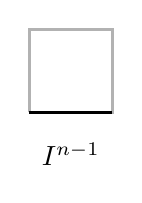
\begin{tikzpicture}[x=3em, y=3em, baseline=1em]
        \draw[very thick, black!30] (0,0)--(1,0)--(1,1)--(0,1)--(0,0);
        \draw[very thick]
        (0,0)--(1,0);
        \filldraw (0.5, -0.5) node{$I^{n-1}$};
    \end{tikzpicture}
    \ar[r, hook]
    &
    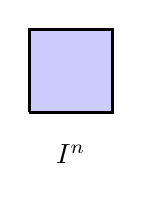
\begin{tikzpicture}[x=3em, y=3em, baseline=1em]
        \filldraw[very thick, fill=blue!20] (0,0)--(1,0)--(1,1)--(0,1)--(0,0);
        \filldraw (0.5, -0.5) node{$I^{n}$};
    \end{tikzpicture}
    & 
    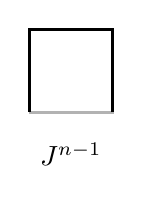
\begin{tikzpicture}[x=3em, y=3em, baseline=1em]
        \draw[very thick, black!30] (0,0)--(1,0)--(1,1)--(0,1)--(0,0);
        \draw[very thick] (1,0)--(1,1)--(0,1)--(0,0);   \filldraw (0.5, -0.5) node{$J^{n-1}$};
    \end{tikzpicture}
    \ar[l, hook]
    \end{tikzcd}
    \)
\end{center}
The \textbf{relative homotopy groups} of the triple $(X,A,x_0)$ are defined as triple homotopy classes of triple maps:
\[\pi_n(X,A,x_0)=[(I^n, I^\ni, J^\ni),(X,A,x_0)].\]
Addition on $\pinr$ for $n\geq 2$ is defined by "juxtaposition and reparametrization in the first coordinate" as follows:
\[[f]+[g]=[f+g],\ (f+g)(\nn{t}{n})=\begin{cases}f(2t_1,\dots,t_n) & t_1\in[0,1/2] \\ g(2t_1-1,\dots,t_n) & t_1\in[1/2,1]\end{cases}\]
this is easily seen to be well defined on homotopy classes.

The \textbf{relative Hurewicz map} is defined similarly to the absolute one: with $c\in H_n(I^n,\de I^n;\Z)$ a generator, define
\[h:\pi_n(X,A,x_0)\to H_n(X,A;\Z),\ [f]\mapsto f_*(c)\]


Recall that $\pi_1(A,x_0)=[(I',\de I'),(A,x_0)]$ acts on $\pi_n(X,A,x_0)$ in a non-trivial fashion. This poses a problem, because for all $[f]\in\pi_n(X,A,x_0)$ and $\omega\in\pi_1(S,x_0)$ the maps representing $[\omega]*[f]$ and $[f]$ are pair-homotopic as maps $(I^n,\de I^n)\to(X,A)$, hence the relative Hurewicz map takes them to the same class in $H_n(X,A;\Z)$.

This leads to the definition of a \textbf{modified relative Hurewicz map}. For $n\geq2$ define $\pinr^\dagger$ to be the quotient of $\pinr$ by the normal subgroup generated by elements of the form $([\omega]*[f])[f]^{-1}$ for all $[\omega]\in\pi_1(A,x_0)$, $[f]\in\pinr$. By design the relative Hurewicz map factors through this quotient:
\begin{center}
    \begin{tikzcd}
        \pinr \arrow[r, "h"] \arrow[d] & \hnr \\
        \pinr^\dagger \arrow[ur, dashed, "h^\dagger" below]
    \end{tikzcd}
\end{center}

Now we can state the relative Hurewicz theorem.

\begin{theorem}[Hurewicz]\label{theorem:hurewicz}
Let $(X,A)$ be a pair of path connected spaces such that for all $x_0\in A$, the map $\pi_1(A,x_0)\to\pi_1(X,x_0)$ is an isomorphism. Let $n\geq2$ and suppose that $\pi_i(X,A,x_0)=0$ for $1\leq i\leq n-1$. Then the modified relative Hurewicz map $h^\dagger$ is an isomorphism.
\end{theorem}

\begin{remark}
For $A=\{x_0\}$, the relative version recovers the absolute version.
\end{remark}

\begin{remark}
The hypothesis of the relative Hurewicz theorem refers to $\pi_i(X,A,x_0)$ but the conclusion refers to $\pi_n(X,A,x_0)^\dagger$. This makes the relative version not as manageable as the absolute one.
\end{remark}